% Options for packages loaded elsewhere
\PassOptionsToPackage{unicode}{hyperref}
\PassOptionsToPackage{hyphens}{url}
\PassOptionsToPackage{dvipsnames,svgnames,x11names}{xcolor}
%
\documentclass[
  letterpaper,
  DIV=11,
  numbers=noendperiod]{scrartcl}

\usepackage{amsmath,amssymb}
\usepackage{iftex}
\ifPDFTeX
  \usepackage[T1]{fontenc}
  \usepackage[utf8]{inputenc}
  \usepackage{textcomp} % provide euro and other symbols
\else % if luatex or xetex
  \usepackage{unicode-math}
  \defaultfontfeatures{Scale=MatchLowercase}
  \defaultfontfeatures[\rmfamily]{Ligatures=TeX,Scale=1}
\fi
\usepackage{lmodern}
\ifPDFTeX\else  
    % xetex/luatex font selection
\fi
% Use upquote if available, for straight quotes in verbatim environments
\IfFileExists{upquote.sty}{\usepackage{upquote}}{}
\IfFileExists{microtype.sty}{% use microtype if available
  \usepackage[]{microtype}
  \UseMicrotypeSet[protrusion]{basicmath} % disable protrusion for tt fonts
}{}
\makeatletter
\@ifundefined{KOMAClassName}{% if non-KOMA class
  \IfFileExists{parskip.sty}{%
    \usepackage{parskip}
  }{% else
    \setlength{\parindent}{0pt}
    \setlength{\parskip}{6pt plus 2pt minus 1pt}}
}{% if KOMA class
  \KOMAoptions{parskip=half}}
\makeatother
\usepackage{xcolor}
\setlength{\emergencystretch}{3em} % prevent overfull lines
\setcounter{secnumdepth}{-\maxdimen} % remove section numbering
% Make \paragraph and \subparagraph free-standing
\makeatletter
\ifx\paragraph\undefined\else
  \let\oldparagraph\paragraph
  \renewcommand{\paragraph}{
    \@ifstar
      \xxxParagraphStar
      \xxxParagraphNoStar
  }
  \newcommand{\xxxParagraphStar}[1]{\oldparagraph*{#1}\mbox{}}
  \newcommand{\xxxParagraphNoStar}[1]{\oldparagraph{#1}\mbox{}}
\fi
\ifx\subparagraph\undefined\else
  \let\oldsubparagraph\subparagraph
  \renewcommand{\subparagraph}{
    \@ifstar
      \xxxSubParagraphStar
      \xxxSubParagraphNoStar
  }
  \newcommand{\xxxSubParagraphStar}[1]{\oldsubparagraph*{#1}\mbox{}}
  \newcommand{\xxxSubParagraphNoStar}[1]{\oldsubparagraph{#1}\mbox{}}
\fi
\makeatother


\providecommand{\tightlist}{%
  \setlength{\itemsep}{0pt}\setlength{\parskip}{0pt}}\usepackage{longtable,booktabs,array}
\usepackage{calc} % for calculating minipage widths
% Correct order of tables after \paragraph or \subparagraph
\usepackage{etoolbox}
\makeatletter
\patchcmd\longtable{\par}{\if@noskipsec\mbox{}\fi\par}{}{}
\makeatother
% Allow footnotes in longtable head/foot
\IfFileExists{footnotehyper.sty}{\usepackage{footnotehyper}}{\usepackage{footnote}}
\makesavenoteenv{longtable}
\usepackage{graphicx}
\makeatletter
\def\maxwidth{\ifdim\Gin@nat@width>\linewidth\linewidth\else\Gin@nat@width\fi}
\def\maxheight{\ifdim\Gin@nat@height>\textheight\textheight\else\Gin@nat@height\fi}
\makeatother
% Scale images if necessary, so that they will not overflow the page
% margins by default, and it is still possible to overwrite the defaults
% using explicit options in \includegraphics[width, height, ...]{}
\setkeys{Gin}{width=\maxwidth,height=\maxheight,keepaspectratio}
% Set default figure placement to htbp
\makeatletter
\def\fps@figure{htbp}
\makeatother

\KOMAoption{captions}{tableheading}
\makeatletter
\@ifpackageloaded{caption}{}{\usepackage{caption}}
\AtBeginDocument{%
\ifdefined\contentsname
  \renewcommand*\contentsname{Table of contents}
\else
  \newcommand\contentsname{Table of contents}
\fi
\ifdefined\listfigurename
  \renewcommand*\listfigurename{List of Figures}
\else
  \newcommand\listfigurename{List of Figures}
\fi
\ifdefined\listtablename
  \renewcommand*\listtablename{List of Tables}
\else
  \newcommand\listtablename{List of Tables}
\fi
\ifdefined\figurename
  \renewcommand*\figurename{Figure}
\else
  \newcommand\figurename{Figure}
\fi
\ifdefined\tablename
  \renewcommand*\tablename{Table}
\else
  \newcommand\tablename{Table}
\fi
}
\@ifpackageloaded{float}{}{\usepackage{float}}
\floatstyle{ruled}
\@ifundefined{c@chapter}{\newfloat{codelisting}{h}{lop}}{\newfloat{codelisting}{h}{lop}[chapter]}
\floatname{codelisting}{Listing}
\newcommand*\listoflistings{\listof{codelisting}{List of Listings}}
\makeatother
\makeatletter
\makeatother
\makeatletter
\@ifpackageloaded{caption}{}{\usepackage{caption}}
\@ifpackageloaded{subcaption}{}{\usepackage{subcaption}}
\makeatother
\makeatletter
\@ifpackageloaded{fontawesome5}{}{\usepackage{fontawesome5}}
\makeatother

\ifLuaTeX
  \usepackage{selnolig}  % disable illegal ligatures
\fi
\usepackage[]{biblatex}
\usepackage{bookmark}

\IfFileExists{xurl.sty}{\usepackage{xurl}}{} % add URL line breaks if available
\urlstyle{same} % disable monospaced font for URLs
\hypersetup{
  pdftitle={Matrix decomposition: Understanding Eigendecomposition - A Fundamental Tool in Linear Algebra},
  pdfauthor={Rafiq Islam},
  colorlinks=true,
  linkcolor={blue},
  filecolor={Maroon},
  citecolor={Blue},
  urlcolor={Blue},
  pdfcreator={LaTeX via pandoc}}


\title{Matrix decomposition: Understanding Eigendecomposition - A
Fundamental Tool in Linear Algebra}
\author{Rafiq Islam}
\date{2025-08-09}

\begin{document}
\maketitle

\renewcommand*\contentsname{Table of contents}
{
\hypersetup{linkcolor=}
\setcounter{tocdepth}{4}
\tableofcontents
}

In many areas of data science, machine learning, and applied
mathematics, \textbf{eigendecomposition} is a core technique for
understanding and transforming data. Whether you're working with
dimensionality reduction (like PCA), solving systems of differential
equations, or analyzing graph structures, chances are you'll run into
eigenvalues and eigenvectors.

\begin{center}\rule{0.5\linewidth}{0.5pt}\end{center}

\subsubsection{What Is
Eigendecomposition?}\label{what-is-eigendecomposition}

Eigendecomposition is a way of \textbf{breaking down} a square matrix
into a set of simpler components based on its \textbf{eigenvalues} and
\textbf{eigenvectors}.

For a given square matrix \(A\), if we can find a basis of eigenvectors,
then \(A\) can be expressed as:

\[
A = Q \Lambda Q^{-1}
\]

Where:

\begin{itemize}
\tightlist
\item
  \(Q\) is a matrix whose columns are the eigenvectors of \(A\).
\item
  \(\Lambda\) (capital lambda) is a \textbf{diagonal matrix} containing
  the eigenvalues of \(A\) along its diagonal.
\item
  \(Q^{-1}\) is the inverse of \(Q\).
\end{itemize}

This is essentially rewriting \(A\) as a combination of \textbf{scaling
operations} along special directions (the eigenvectors).

\subsubsection{Eigenvalues and Eigenvectors
Recap}\label{eigenvalues-and-eigenvectors-recap}

Before decomposition, we need to understand the building blocks:

Given a square matrix \(A\), an \textbf{eigenvector} \(\mathbf{v}\) and
\textbf{eigenvalue} \(\lambda\) satisfy:

\[
A \mathbf{v} = \lambda \mathbf{v}
\]

\begin{itemize}
\tightlist
\item
  \(\mathbf{v}\) is a direction in which the transformation \(A\) acts
  by \textbf{stretching or compressing} without rotating it.
\item
  \(\lambda\) tells us how much \(A\) scales \(\mathbf{v}\).
\end{itemize}

Example: If \(A \mathbf{v} = 3 \mathbf{v}\), then \(\mathbf{v}\) is
scaled by a factor of 3 under \(A\).

\subsubsection{When Can We Use
Eigendecomposition?}\label{when-can-we-use-eigendecomposition}

Not all matrices can be decomposed this way.

\begin{itemize}
\tightlist
\item
  Eigendecomposition is possible for \textbf{diagonalizable matrices},
  i.e., matrices with enough linearly independent eigenvectors to form a
  basis.
\item
  \textbf{Symmetric matrices} (in real-valued cases) are always
  diagonalizable and have orthogonal eigenvectors.
\end{itemize}

If a matrix is \textbf{defective} (doesn't have enough eigenvectors), we
can't use eigendecomposition directly --- but other decompositions (like
Jordan decomposition or SVD) still work.

\subsubsection{Why Is This Useful?}\label{why-is-this-useful}

Eigendecomposition lets us \textbf{simplify matrix operations} by
working in a new coordinate system defined by eigenvectors.

If:

\[
A = Q \Lambda Q^{-1}
\]

Then:

\[
A^k = Q \Lambda^k Q^{-1}
\]

Where \(\Lambda^k\) is just the diagonal matrix with each eigenvalue
raised to the \(k\)-th power. This makes repeated multiplications or
exponentials of matrices much easier.

\subsubsection{Applications in Data Science and
Beyond}\label{applications-in-data-science-and-beyond}

\paragraph{\texorpdfstring{\textbf{Principal Component Analysis
(PCA)}}{Principal Component Analysis (PCA)}}\label{principal-component-analysis-pca}

\begin{itemize}
\tightlist
\item
  PCA uses eigendecomposition of the covariance matrix to find the
  \textbf{principal directions} of data variability.
\item
  Eigenvectors correspond to directions of maximum variance; eigenvalues
  tell you how much variance is captured.
\end{itemize}

\paragraph{\texorpdfstring{\textbf{Solving Systems of Differential
Equations}}{Solving Systems of Differential Equations}}\label{solving-systems-of-differential-equations}

\begin{itemize}
\tightlist
\item
  Linear ODE systems can be solved by diagonalizing the system matrix.
\end{itemize}

\paragraph{\texorpdfstring{\textbf{Graph
Analysis}}{Graph Analysis}}\label{graph-analysis}

\begin{itemize}
\tightlist
\item
  In spectral graph theory, eigenvalues of adjacency or Laplacian
  matrices reveal connectivity and clustering properties.
\end{itemize}

\paragraph{\texorpdfstring{\textbf{Markov
Chains}}{Markov Chains}}\label{markov-chains}

\begin{itemize}
\tightlist
\item
  The steady state of a Markov process is related to the eigenvector
  corresponding to eigenvalue \(\lambda = 1\).
\end{itemize}

\begin{center}\rule{0.5\linewidth}{0.5pt}\end{center}

\subsubsection{A Simple Example}\label{a-simple-example}

Let's take:

\[
A = \begin{bmatrix} 4 & 1 \\ 2 & 3 \end{bmatrix}
\]

\begin{enumerate}
\def\labelenumi{\arabic{enumi}.}
\tightlist
\item
  \textbf{Find eigenvalues} by solving:
\end{enumerate}

\[
\det(A - \lambda I) = 0
\]

\[
(4 - \lambda)(3 - \lambda) - 2 = \lambda^2 - 7\lambda + 10 = 0
\]

\[
\lambda_1 = 5, \quad \lambda_2 = 2
\]

\begin{enumerate}
\def\labelenumi{\arabic{enumi}.}
\setcounter{enumi}{1}
\tightlist
\item
  \textbf{Find eigenvectors} by solving
  \((A - \lambda I)\mathbf{v} = 0\).
\end{enumerate}

\begin{itemize}
\tightlist
\item
  For \(\lambda = 5\): eigenvector \(\mathbf{v}_1 = [1, 1]^T\)
\item
  For \(\lambda = 2\): eigenvector \(\mathbf{v}_2 = [-1, 2]^T\)
\end{itemize}

\begin{enumerate}
\def\labelenumi{\arabic{enumi}.}
\setcounter{enumi}{2}
\tightlist
\item
  \textbf{Form Q and Λ}:
\end{enumerate}

\[
Q = \begin{bmatrix} 1 & -1 \\ 1 & 2 \end{bmatrix}, \quad
\Lambda = \begin{bmatrix} 5 & 0 \\ 0 & 2 \end{bmatrix}
\]

\begin{enumerate}
\def\labelenumi{\arabic{enumi}.}
\setcounter{enumi}{3}
\tightlist
\item
  \textbf{Check}:
\end{enumerate}

\[
A = Q \Lambda Q^{-1}
\]

\begin{center}\rule{0.5\linewidth}{0.5pt}\end{center}

\subsubsection{Visualization.}\label{visualization.}

\begin{center}
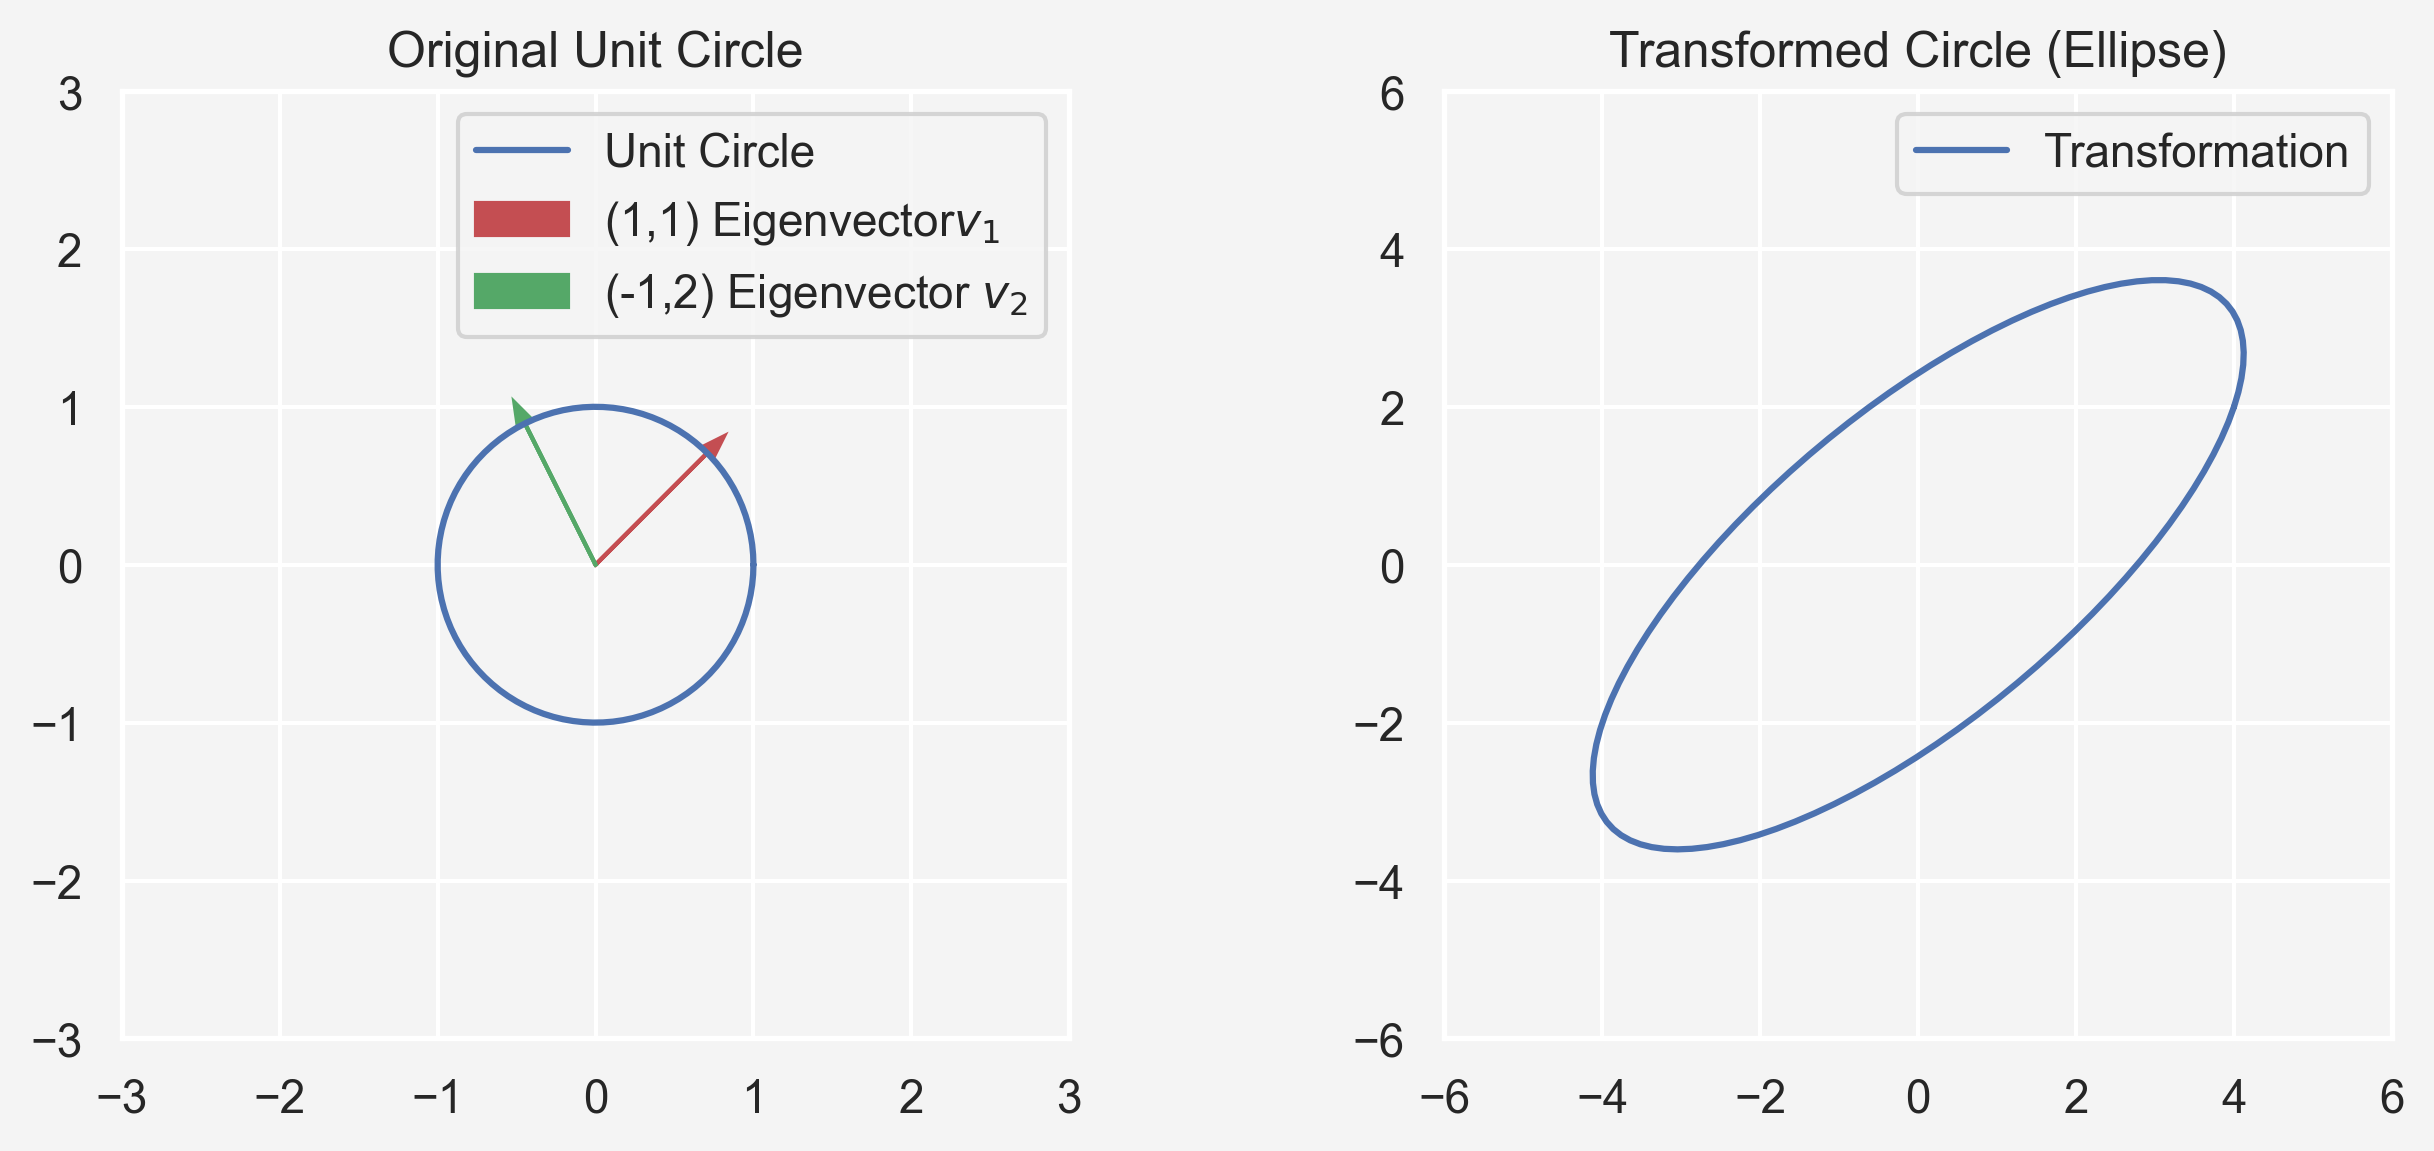
\includegraphics{index_files/figure-pdf/cell-2-output-1.png}
\end{center}

\subsubsection{Key Takeaways}\label{key-takeaways}

\begin{itemize}
\tightlist
\item
  \textbf{Eigendecomposition = diagonalization} of a matrix via
  eigenvalues and eigenvectors.
\item
  Only works for diagonalizable matrices, but symmetric matrices are
  guaranteed to work.
\item
  Simplifies many computations, from raising matrices to powers to
  solving ODEs.
\item
  Foundation for PCA, spectral graph analysis, and many machine learning
  methods.
\end{itemize}

\begin{center}\rule{0.5\linewidth}{0.5pt}\end{center}

💡 \textbf{Tip:} If your matrix isn't diagonalizable, try
\textbf{Singular Value Decomposition (SVD)} --- it works for any matrix
and generalizes many of the benefits of eigendecomposition.

\textbf{Share on}

\faIcon{facebook}

\faIcon{linkedin}

\faIcon{twitter}

\phantomsection\label{fb-root}

\textbf{You may also like}


\printbibliography



\end{document}
